\documentclass{article}

\usepackage{graphicx}
\usepackage{tikz}
\usepackage{tikzsymbols}
\usetikzlibrary{calc,patterns,shapes.geometric}
\pagestyle{empty}
\usepackage[margin=0pt]{geometry}
\geometry{papersize={14in,12in}}

\def\centerarc[#1](#2)(#3:#4:#5){\draw[#1] ($(#2)+({#5*cos(#3)},{#5*sin(#3)})$) arc (#3:#4:#5);}

\begin{document}
	\begin{figure}
		\centering
		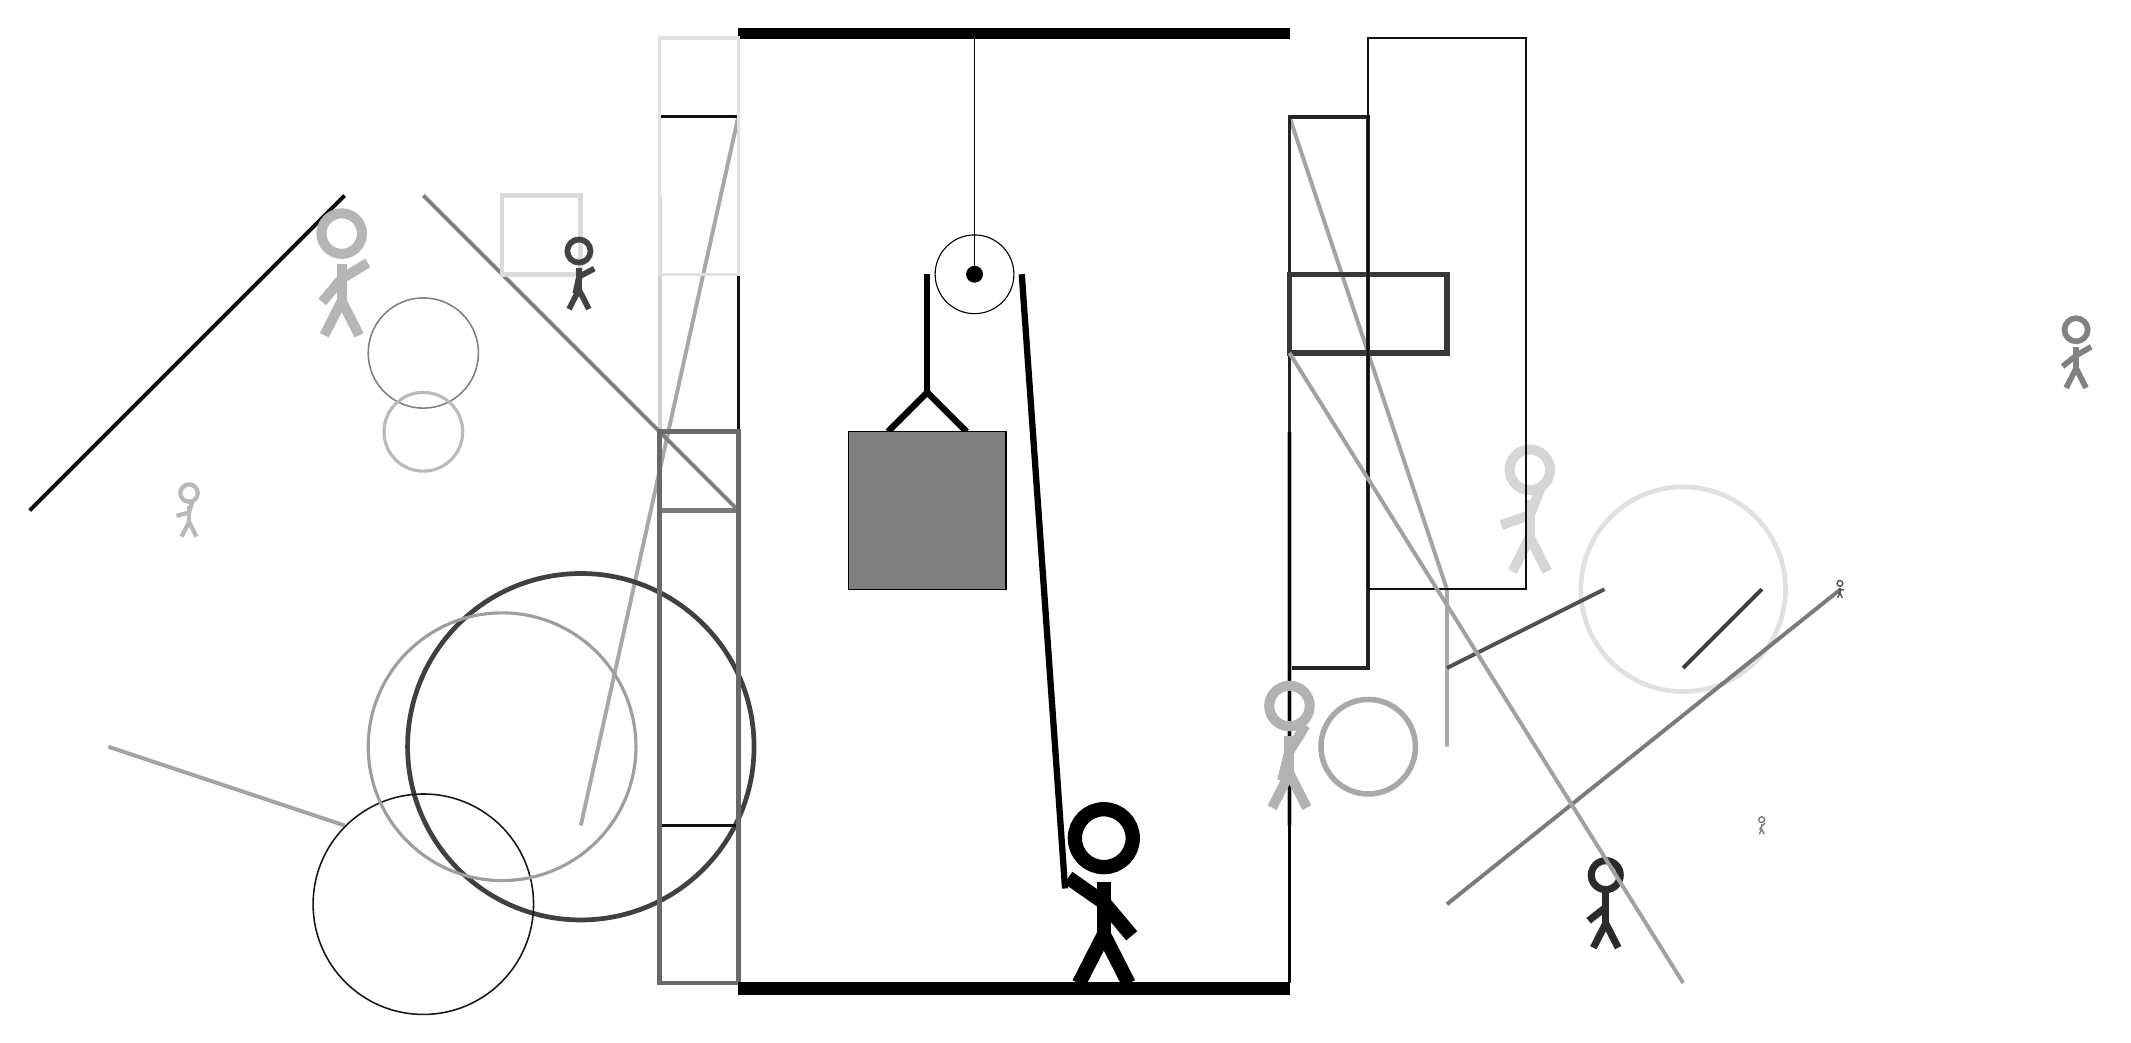
\begin{tikzpicture}
			%%%%% START %%%%%
			
			\draw[fill=black] (-2, 9) rectangle (5, 9.125);
			
			\draw[line width=0.5mm, color=black!34](-2, 8) -- (-4, -1);
			
			\draw [line width=0.6mm, color=black!75](-4, 0) circle (2.2);
			\draw[line width=0.5mm, color=black!76](10, 1) -- (11, 2);
			\draw[line width=0.5mm, color=black!36](5, 8) -- (7, 2);
			\draw[line width=0.5mm, color=black!34] (7, 2) rectangle (7, 0);
			\draw[line width=0.5mm, color=black!86] (5, 8) rectangle (6, 1);
			\draw [line width=0.6mm, color=black!12](10, 2) circle (1.3);
			\draw[line width=0.6mm, color=black!29] (5, -1) rectangle (5, 4);
			\draw [line width=0.7mm, color=black!34](6, 0) circle (0.6);
			
			\draw [line width=0.3mm, color=black!76](7, 2) circle (0.0);
			
			\draw[line width=0.7mm, color=black!78] (7, 5) rectangle (5, 6);
			\node[line width=0.7mm, color=black!49] at (15, 5) {\Strichmaxerl[4][39][30]};
			\node[line width=0.5mm, color=black!83] at (9, -2) {\Strichmaxerl[5][38][90]};
			
			\draw[line width=0.5mm, color=black!52](7, -2) -- (12, 2);
			\draw[line width=0.5mm, color=black!36](-7, -1) -- (-10, 0);
			\draw[line width=0.5mm, color=black!98] (5, -3) rectangle (5, 4);
			
			\draw [line width=0.2mm, color=black!50](-6, 5) circle (0.7);
			
			\draw[line width=0.4mm, color=black!94] (-2, -1) rectangle (-3, 8);
			\draw[line width=0.5mm, color=black!95](-7, 7) -- (-11, 3);
			\node[line width=0.4mm, color=black!51] at (11, -1) {\Strichmaxerl[1][60][40]};
			\node[line width=0.6mm, color=black!66] at (12, 2) {\Strichmaxerl[1][74][4]};
			
			\draw[line width=0.5mm, color=black!18] (-3, 7) rectangle (-3, 4);
			
			\node[line width=0.3mm, color=black!16] at (8, 3) {\Strichmaxerl[7][20][68]};
			\node[line width=0.4mm, color=black!30] at (5, 0) {\Strichmaxerl[7][76][58]};
			\draw[line width=0.5mm, color=black!50](-2, 3) -- (-6, 7);
			
			\draw[line width=0.5mm, color=black!68](7, 1) -- (9, 2);
			\draw[line width=0.4mm, color=black!12] (-3, 9) rectangle (-2, 6);
			\draw[line width=0.6mm, color=black!14] (-4, 6) rectangle (-5, 7);
			\draw[line width=0.3mm, color=black!94] (6, 9) rectangle (8, 2);
			
			\draw[line width=0.6mm, color=black!52] (-3, 3) rectangle (-2, 3);
			\node[line width=0.3mm, color=black!28] at (-9, 3) {\Strichmaxerl[3][16][73]};
			
			\node[line width=0.6mm, color=black!29] at (-7, 6) {\Strichmaxerl[7][50][31]};
			\draw [line width=0.2mm, color=black!91](-6, -2) circle (1.4);
			
			\draw [line width=0.4mm, color=black!27](-6, 4) circle (0.5);
			\node[line width=0.6mm, color=black!74] at (-4, 6) {\Strichmaxerl[4][78][28]};
			\draw [line width=0.4mm, color=black!38](-5, 0) circle (1.7);
			\draw[line width=0.5mm, color=black!37](10, -3) -- (5, 5);
			\draw[line width=0.6mm, color=black!59] (-3, 4) rectangle (-2, -3);
			
			\draw (1, 6) circle (0.5);
			\draw[fill=black] (1, 6) circle (0.1);
			\draw (1, 9) -- (1, 6);
			
			\draw[line width=0.8mm] (-0.1, 4.0) -- (0.4, 4.5) -- (0.9, 4.0);
			\draw[fill=black!50] (-0.6, 4.0) rectangle (1.4, 2.0);
			
			\draw[line width=0.8mm] (0.4, 6) -- (0.4, 4.5);
			\centerarc[line width=0.8mm](1, 6)(0:180:0.6);
			\draw[line width=0.8mm](1.6, 6) -- (2.15, -1.8);
			
			\node at (2.6, -1.9) {\Strichmaxerl[10][-35][-50]};
			
			\draw[fill=black] (-2, -3) rectangle (5, -3.15);
			
			%%%%% END %%%%%
		\end{tikzpicture}
	\end{figure}	
\end{document}